\documentclass{report}
\usepackage[margin=1in, paperwidth=8.5in, paperheight=11in]{geometry}
%Math packages%
\usepackage{amsmath}
\usepackage{amsthm}
%Spacing%
\usepackage{setspace}
\onehalfspacing
%Lecture number%
\newcommand{\lectureNum}{2}
%Variables - Date and Course%
\newcommand{\curDate}{January 6, 2017}
\newcommand{\course}{MATH 239}
\newcommand{\instructor}{Luke Postle}
%Defining the example tag%
%\theoremstyle{definition}%
\newtheorem{ex}{Example}[section]
%Setting counter given the lecture number%
\setcounter{chapter}{\lectureNum{}}
%Package for drawing graphs%
\usepackage{tikz}
\usepackage{verbatim}
\usetikzlibrary{arrows}

\begin{document}
%Note title%
\begin{center}
\begin{Large}
\textsc{\course{} | Lecture \lectureNum{}}
\end{Large}
\end{center} 
\noindent \textit{Bartosz Antczak} \hfill
\textit{Instructor: \instructor{}} \hfill
\textit{\curDate{}}
\rule{\textwidth}{0.4pt}

% Actual Notes%
\subsubsection{Review of last lecture}
A \textbf{graph} is a set of of elements called \textbf{vertices} with a set of distinct pairs of vertices called \textbf{edges}. Some examples of graphs we've covered include:
\begin{itemize}
\item Complete ($K_n$)
\item Cycle ($C_n$)
\item Path ($P_n$)
\item Complete bipartite graph ($K_{m,\,n}$, also called \textit{cliques})
\end{itemize}

\section{Notation and terminology}
$V(G)$ denotes the set of vertices on a graph $G$, and $E(G)$ denotes the set of edges. If $\{uv\} \in E(G)$ (NOTE: we can also denote $\{uv\}$ without the brackets, simply as $uv$), then we say $u$ is \underline{adjacent} to $v$, and we also say that $v$ is a \underline{neighbour} of $u$.\\
If $v \in V(G)$, we let $N(v)$ denote the \underline{neighbourhood} of $v$, which is the set of neighbours of $v$. The number of neighbours of $v$, which is $\vert N(v) \vert$, is called the \underline{degree} of $v$.\\
If $e = uv$ is an edge of $G$, then we say that $u$ and $v$ are the \underline{ends} of $e$. Furthermore, we say $e$ is \underline{incident} with $u$ or $v$ and similarly $u$ or $v$ is incident with $e$. We also say two edges $e_1$ and $e_2$ are incident if they have a common end.

\subsection{Definition: subgraph}
A \textbf{subgraph} $H$ of $G$ is a graph such that $V(H) \subseteq V(G)$ and $E(H) \subseteq E(G)$, or equivalently, $H$ can be obtained from $G$ by deleting some vertices (and all incident edges) and some additional edges.
\begin{ex}
$\forall \, m \leq n$, $K_m$ is a subgraph of $K_n$. Actually, every graph on at most $n$ vertices is a subgraph of $K_n$
\end{ex}
\noindent Also, the only subgraph of $C_n$ is $C_n$ itself! What about $P_m$? $P_m$ is a subgraph of $N_n$, $\forall \, m \leq n$.
\subsubsection{Deleting edges and vertices}
If $v \in  V(G)$, we let $G - v$ denote the graph obtained from $G$ by deleting $v$ and all incident edges.\\
If $e \in  E(G)$, we let $G - e$ denote the graph obtained from $G$ by deleting $e$.
\newpage
\section{Graph properties}
We define graphs based on their properties, some examples include:
\begin{itemize}
\item Having a certain number of vertices (or edges)
\item Having a vertex of degree 1
\item Containing a triangle as a subgraph
\item Having no cycle as a subgraph
\end{itemize}
One property we'll focus on is whether a graph is \textit{bipartite}.
\subsection{Definition: bipartite}
A graph $G$ is \textbf{bipartite} if there exists a partition of $V(G)$ into two disjoints $A$ and $B$ such that every edge of $G$ has exactly one end in $A$ and the other in $B$. Some examples include:
\begin{itemize}
\item $K_{m,\,n}$, $\forall\,m,m$
\item $P_z$, $\forall\,z$
\item $K_1$ and $K_2$; however, $K_3$ isn't bipartite! Let's prove it:
\end{itemize}

\subsubsection{Proof}
Proof by contradiction.\\
Suppose that $K_3$ is bipartite. This means that there exists a partition $A,\,B$ of $V(G)$ with all edges with one in $A$ and other in $B$. Note that at least one of $A$ or $B$ has size at least 2, because of the \textit{pigeonhole principle}\footnote{$m$ pigeons into $n$ holes. If $m > n$, then there exists a hole with at least 2 pigeons.}.\\
Now suppose without loss of generality (abbreviated to ``wlog"), that $\vert A \vert = 2$. Let $u, v \in A$. Since $K_3$ is complete, $uw \in E(G)$ with both ends in $A$ | a contradiction.\\\\
So what other graphs are not bipartite? Well, $C_n$ where $n$ is odd is not bipartite. Actually, any graph that contains a triangle is not bipartite. Why? Well it's because of a proposition: if $H$ is a subgraph of $G$ and $G$ is bipartite, then so is $H$.

\subsubsection{Question to finish this lecture}
How do we know that two graphs are the same (are equal)? For example, $C_4 = K_{2,2}$:

%Graph 1%
\begin{center}
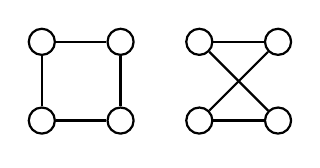
\begin{tikzpicture}[-,auto,node distance=1cm,
                    thick,main node/.style={circle,draw,font=\sffamily\small}]
  %C_4%
  \node[main node] (1) {};
  \node[main node] (2) [right of=1] {};
  \node[main node] (3) [below of=2] {};
  \node[main node] (4) [left of=3] {};
  %K_{2,2}%
  \node[main node] (5)[right of=2] {};
  \node[main node] (6)[right of=5] {};
  \node[main node] (7)[below of=6] {};
  \node[main node] (8)[left of=7] {};
  
  \path[every node/.style={font=\sffamily\small}]
    (1) edge node [left] {} (2)
    	edge node [below] {} (4)
    (3) edge node [left] {} (2)
    	edge node[below] {} (4)
    (5) edge node [left] {} (6)
    	edge node [below] {} (7)
    (8) edge node [left] {} (6)
    	edge node[below] {} (7);
\end{tikzpicture}
\end{center}
Notice that these graphs are visually different, but the definition of graphs doesn't concern how they look like. Why are they equal? Because there exists a \textit{bijection} between the vertex sets. More on this in the next lecture!
%END%
\end{document}